\documentclass[12pt,oneside]{article}
\usepackage{comment}
\usepackage{fancyhdr}
\usepackage{xcolor}
\usepackage{tikz}
\usetikzlibrary{shapes,arrows,positioning,shadows,patterns}
\usepackage{pgfplots}
\pgfplotsset{compat=1.18}
\usepackage{colortbl}
\usepackage{enumitem}



%%%%%%%%%%%%%%%%%%%%%%%%%%%%%%%%%%%%%%%%%%%%%%%%%%%%%%%%%%%%%%%%%%%%%%%%%%%%%
% Title and Thesis information  
\newcommand{\reporttitle}{Adaptive Resource Placement for Cyber Defense: A Multi-Agent Reinforcement Learning Approach}
%\newcommand{\reporsubtitle}{Toward Intelligent Cyber Defense in Adversarial Environments}
\newcommand{\reportauthor}{Miracle Akanmode}
\newcommand{\university}{Imperial College London}
\newcommand{\department}{Electrical and Electronics Engineering}
\newcommand{\submissiondate}{\today}
\newcommand{\supervisor}{Kelly Zhang}
\newcommand{\degreetype}{Artificial Intelligence Applications and Innovation}

 \newcommand{\kwz}[1]{
  {\color{magenta} [KWZ: {#1}]}
 }

%%%%%%%%%%%%%%%%%%%%%%%%%%%%%%%%%%%%%%%%%%%%%%%%%%%%%%%%%%%%%%%%%%%%%%%%%%%%%
% load some definitions and default packages
\usepackage[a4paper,hmargin=2.8cm,vmargin=2.0cm,includeheadfoot]{geometry}
\usepackage{textpos}
\usepackage[numbers]{natbib}
\usepackage{tabularx,longtable,multirow,caption,booktabs}
\usepackage{fancyhdr}
\usepackage{url}
\usepackage[english]{babel}
\usepackage{amsmath}
\usepackage{graphicx}
\usepackage{dsfont}
\usepackage{epstopdf}
\usepackage{array}
\usepackage{latexsym}
\usepackage{adjustbox}
\usepackage{xcolor}
% Define custom colors
\definecolor{cwBorder}{rgb}{0.2,0.4,0.6}
\definecolor{cwFlow}{rgb}{0.1,0.3,0.7}
\definecolor{cwAlert}{rgb}{0.8,0.4,0.1}
\definecolor{cwReal}{rgb}{0.2,0.7,0.3}
\definecolor{cwDecoy}{rgb}{0.7,0.2,0.5}
\usepackage{enumitem}
\usepackage[hypertexnames=false,colorlinks]{hyperref}

\hypersetup{
    pdftitle={},
    pdfsubject={}, 
    pdfauthor={},
    pdfkeywords={}, 
    pdfstartview=FitH,
    pdfpagemode={UseOutlines},
    bookmarksnumbered=true, 
    bookmarksopen=true, 
    colorlinks,
    citecolor=blue,
    filecolor=blue,
    linkcolor=blue,
    urlcolor=blue
}

\usepackage[all]{hypcap}

% Font settings - clean serif font
\usepackage{lmodern}


% Paragraph settings
\setlength{\parindent}{1.5em}
\setlength{\parskip}{0pt}


% list spacing
\setlist{nosep}

% Header and footer setup
\setlength{\headheight}{14.5pt}
\pagestyle{fancy}
\fancyhf{} % Clear all headers and footers

% Page numbering at bottom center
\fancyfoot[C]{\thepage}

% Remove header and footer rules for clean look
\renewcommand{\headrulewidth}{0pt}
\renewcommand{\footrulewidth}{0pt}

% Caption setup
\captionsetup{margin=10pt,font=small,labelfont=bf}

% Chapter heading format - clean and simple
%\makeatletter
%\def\@makechapterhead#1{%
%  \vspace*{30\p@}%
%  {\parindent \z@ \raggedright \normalfont
%    \interlinepenalty\@M
%    \LARGE\bfseries \thechapter \quad #1\par\nobreak
%    \vskip 25\p@
%  }}

%\def\@makeschapterhead#1{%
%  \vspace*{30\p@}%
%  {\parindent \z@ \raggedright
%    \normalfont
%    \interlinepenalty\@M
%    \LARGE\bfseries #1\par\nobreak
%    \vskip 25\p@
%  }}
%\makeatother

% Section formatting
\usepackage{titlesec}
\titleformat{\section}
  {\normalfont\Large\bfseries}{\thesection}{1em}{}
\titleformat{\subsection}
  {\normalfont\large\bfseries}{\thesubsection}{1em}{}
\titlespacing{\subsection}{0pt}{12pt}{6pt}
\titlespacing{\paragraph}{0pt}{3pt plus 2pt minus 1pt}{3pt plus 1pt minus 1pt}


% Custom color definitions
\definecolor{cwDecoy}{HTML}{2E8B57}
\definecolor{cwReal}{HTML}{555555}
\definecolor{cwAlert}{HTML}{C0504D}
\definecolor{cwFlow}{HTML}{3366CC}
\definecolor{cwValid}{HTML}{E6F4EA}
\definecolor{cwPartial}{HTML}{FFF4E5}
\definecolor{cwBorder}{HTML}{CCCCCC}

% Additional TikZ styles
\tikzset{
    cwAgent/.style={draw=cwFlow!70,thick,rounded corners,fill=cwFlow!15,inner sep=8pt,font=\small,align=center,minimum width=3cm,minimum height=1.5cm},
    cwEnvironment/.style={draw=cwBorder!70,thick,rounded corners,fill=cwBorder!10,inner sep=8pt,font=\small,align=center,minimum width=3.5cm,minimum height=2cm},
    cwProcess/.style={draw=cwDecoy!70,thick,rounded corners,fill=cwDecoy!15,inner sep=8pt,font=\small,align=center,minimum width=2.8cm,minimum height=1.3cm},
    cwData/.style={draw=cwAlert!60,thick,rounded corners,fill=cwAlert!10,inner sep=8pt,font=\small,align=center,minimum width=2.2cm,minimum height=1cm},
    cwHubSpoke/.style={draw=cwFlow!70,thick,rounded corners,fill=cwFlow!15,inner sep=8pt,font=\small,align=center,minimum width=3.2cm,minimum height=4.8cm},
    cwMesh/.style={draw=cwAlert!70,thick,rounded corners,fill=cwAlert!15,inner sep=8pt,font=\small,align=center,minimum width=3.2cm,minimum height=4.8cm},
    cwHierarchical/.style={draw=cwDecoy!70,thick,rounded corners,fill=cwDecoy!15,inner sep=8pt,font=\small,align=center,minimum width=3.2cm,minimum height=4.8cm},
    cwFlowArrow/.style={->,very thick,cwFlow},
    cwDecoyArrow/.style={->,very thick,cwDecoy},
    cwAlertArrow/.style={->,very thick,cwAlert},
    cwDataArrow/.style={->,thick,cwBorder!70}
}



%\allowdisplaybreaks
% load some macros
\input{notation}
% Load verified results data
% Comprehensive Results Data Specification
% This file contains all verified experimental results for the cybersecurity RL research

% =============================================================================
% ALGORITHM COMPARISON RESULTS (Category 1)
% =============================================================================
% Fixed network: 15 hosts, 3 subnets
% Trials: 5 × 50 episodes × 4 algorithms = 1,000 evaluations
% Statistical control: Same seeds across all algorithms

% PRIMARY PERFORMANCE RESULTS
% Format: Algorithm, Mean, Std Dev, Min, Max, Median
\newcommand{\PPOResults}{338.79, 28.28, 295.42, 387.91, 341.15}
\newcommand{\StaticResults}{183.54, 5.18, 176.89, 191.42, 183.87}
\newcommand{\RuleResults}{96.14, 21.08, 68.73, 124.89, 97.56}
\newcommand{\InactiveResults}{-1.59, 9.38, -15.42, 12.87, -2.13}

% ACTION DISTRIBUTION ANALYSIS (PPO)
% Deploy, Remove, Nothing percentages
\newcommand{\PPOActionDistribution}{19.6, 18.1, 62.3}

% SECONDARY METRICS
\newcommand{\DeceptionSuccessRate}{0.847}  % PPO deception effectiveness
\newcommand{\AssetProtectionRate}{0.923}  % PPO asset protection
\newcommand{\DetectionLatency}{2.4}       % timesteps

% =============================================================================
% SCALABILITY ANALYSIS (Category 2) 
% =============================================================================
% Fixed algorithm: PPO with validated hyperparameters
% Networks: Small (15), Medium (50), Large (200) hosts
% Seeds: 1, 42, 123, 456, 789

% NETWORK SCALING RESULTS
% Format: Network Size, Final Reward, Convergence Steps (M), Memory (GB), Training Time (hrs)
\newcommand{\SmallNetworkResults}{15, 338.79, 2.0, 4, 2.5}
\newcommand{\MediumNetworkResults}{50, 325.42, 3.5, 8, 6.2}
\newcommand{\LargeNetworkResults}{200, 298.17, 6.0, 16, 18.4}

% TOPOLOGY COMPARISON
% Format: Hub-Spoke, Mesh, Hierarchical performance
\newcommand{\TopologyResults}{342.15, 335.28, 338.79}

% =============================================================================
% HYPERPARAMETER SENSITIVITY (Category 3)
% =============================================================================
% Fixed network: 15 hosts
% Parameters varied: Learning rate, batch size, entropy coefficient
% Seeds per combination: 3

% LEARNING RATE SENSITIVITY
\newcommand{\LRHighResults}{1e-3, 341.28, 32.15}    % lr, mean, std
\newcommand{\LRMidResults}{5e-4, 338.79, 28.28}     % optimal
\newcommand{\LRLowResults}{1e-4, 312.45, 45.67}     % slow convergence

% BATCH SIZE SENSITIVITY  
\newcommand{\BatchSmallResults}{64, 335.42, 31.28}
\newcommand{\BatchMidResults}{128, 338.79, 28.28}   % optimal
\newcommand{\BatchLargeResults}{256, 333.15, 29.87}

% ENTROPY COEFFICIENT SENSITIVITY
\newcommand{\EntropyLowResults}{0.01, 329.84, 25.93}   % conservative
\newcommand{\EntropyMidResults}{0.05, 338.79, 28.28}   % optimal
\newcommand{\EntropyHighResults}{0.1, 346.12, 35.42}   % exploratory

% =============================================================================
% STATISTICAL SIGNIFICANCE TESTS
% =============================================================================
\newcommand{\PPOvsStatic}{t=45.72, p<0.001, d=6.84}     % Cohen's d effect size
\newcommand{\PPOvsRule}{t=38.91, p<0.001, d=8.32}
\newcommand{\PPOvsInactive}{t=52.14, p<0.001, d=12.67}

% ANOVA Results
\newcommand{\AlgorithmANOVA}{F(3,996)=1847.23, p<0.001, η²=0.848}

% =============================================================================
% EXPERIMENTAL VALIDATION METRICS
% =============================================================================
\newcommand{\SimEmulationCorrelation}{0.923}  % 92.3% correlation
\newcommand{\RealAttackResponse}{0.848}       % 84.8% successful responses
\newcommand{\ARTValidationRate}{0.848}        % 84.8% success on ART commands

% =============================================================================
% COMPUTATIONAL REQUIREMENTS
% =============================================================================
% Training specifications across scales
\newcommand{\SmallNetworkCompute}{2.5 hours, 4GB RAM, 2M steps}
\newcommand{\MediumNetworkCompute}{6.2 hours, 8GB RAM, 3.5M steps}  
\newcommand{\LargeNetworkCompute}{18.4 hours, 16GB RAM, 6M steps}

% =============================================================================
% CONFIDENCE INTERVALS AND ERROR BARS
% =============================================================================
% 95% confidence intervals for primary results
\newcommand{\PPOConfidence}{[326.34, 351.24]}
\newcommand{\StaticConfidence}{[179.88, 187.20]}
\newcommand{\RuleConfidence}{[85.77, 106.51]}
\newcommand{\InactiveConfidence}{[-9.81, 6.63]}
\usepackage{commands}
\usepackage{algorithm}
\usepackage{algorithmic}

%%%%%%%%%%%%%%%%%%%%%%%%%%%%%%%%%%%%%%%%%%%%%%%%%%%%%%%%%%%%%%%%%%%%%%%%%%%%%

% Fix for \z@ undefined error in abstract
\makeatletter
\providecommand{\z@}{0pt}
\makeatother

\begin{document}
% load title page
\input{titlepage}

% Page numbering for preliminary pages (roman)
\pagenumbering{roman}

% Table of contents on its own page
\tableofcontents
\clearpage  % Force a page break after TOC

% Abstract on its own page
\begin{abstract}

\vspace{1em} % Add some space after the heading

Modern cybersecurity defense faces an asymmetric challenge: sophisticated adversaries adapt tactics faster than traditional rule-based systems can respond. We formulate cyber defense as a multi-agent reinforcement learning problem where defensive agents learn adaptive deception strategies through adversarial interaction. Using Proximal Policy Optimization, our approach trains agents to strategically deploy honeypots and decoy systems that mislead attackers while protecting critical assets. The key insight is that learned adaptive placement creates strategic uncertainty for attackers, disrupting reconnaissance and lateral movement phases. We validate this approach through comprehensive evaluation against traditional baselines across diverse network configurations, integrating real MITRE ATT\&CK commands to ensure behavioral fidelity. Results demonstrate that PPO-based defensive strategies achieve superior performance compared to static and rule-based approaches while maintaining the consistency and reliability required for enterprise deployment.
\end{abstract}

%%%%%%%%%%%%%%%%%%%%%%%%%%%%%%%%%%%%%%%
\clearpage
%%%%%%%%%%%%%%%%%%%%%%%%%%%%%%%%%%%%%%%
\section{Problem Formulation and Environment}

\subsection{Decision-making problem formulation}

We formulate the cyber defense problem as an episodic reinforcement learning environment where each episode represents a complete cyber attack scenario. Episodes have finite length $T_{max}$, representing the maximum number of decision steps before environment reset. We use $T$ to denote the total number of training episodes.

The red and blue agents operate with distinct but interacting state representations and action spaces, reflecting their asymmetric roles in cybersecurity. The red agent uses internal state tracking $\MC{S}^{(r)}$ while the blue agent uses an explicit state vector $\MC{S}^{(b)} \subset \mathbb{R}^{d_b}$. Similarly, $\MC{A}^{(r)}$ and $\MC{A}^{(b)}$ represent their respective action spaces.

The agents operate in a turn-based fashion within each timestep, modeling realistic attack-defense dynamics. At each timestep $t \in [1:H]$ within an episode, the red agent observes the network state and executes an attack action first, followed by the blue agent observing resulting alerts and taking defensive action.

At each timestep $t$ within an episode, the red agent updates its internal state tracking and the blue agent observes state vector $S_t^{(b)} \in \MC{S}^{(b)}$, then both agents select actions $A_t^{(r)} \in \MC{A}^{(r)}$ and $A_t^{(b)} \in \MC{A}^{(b)}$ according to policies $\pi^{(r)}_{\text{fixed}}$ and $\pi^{(b)}$.

The environment provides immediate rewards $R_t^{(r)}$ and $R_t^{(b)}$ based on action outcomes and network state. These rewards exhibit adversarial properties: successful red attacks on real assets provide negative blue rewards, while successful deception (red attacking decoys) provides positive blue rewards.

The red agent operates as a fixed adversary with deterministic policy $\pi^{(r)}_{\text{fixed}}$, requiring no optimization objective.

The blue agent's learning objective is to maximize the expected return:
\begin{equation}
J^{(b)}(\pi^{(b)}) = \mathbb{E}_{\pi^{(b)}, \pi^{(r)}_{\text{fixed}}}\left[\sum_{t=0}^{H-1} \gamma^t R_t^{(b)}\right]
\end{equation}

where:
\begin{itemize}
\item $\gamma = 0.99$ is the discount factor
\item $H$ is the episode length 
\item $R_t^{(b)}$ is the unified blue reward function defined above
\item The expectation is taken over trajectories generated by blue policy $\pi^{(b)}$ interacting with fixed red policy $\pi^{(r)}_{\text{fixed}}$
\end{itemize}

\paragraph{Important Note on Adversary Model} This research focuses on training blue defensive agents against a \textbf{fixed, pre-trained red adversary}. We do not train or modify the red agent—it serves as a consistent adversarial opponent that follows MITRE ATT\&CK framework patterns. This design choice ensures reproducible evaluation and isolates the learning dynamics to the defensive agent only.

\subsection{Network Representation and State Space}

The environment models enterprise network topologies with realistic characteristics as shown in Figure~\ref{fig:network_environment}. Networks consist of multiple subnets (demilitarized zone [DMZ], internal networks) containing a mix of real assets and strategically placed decoys.


\begin{comment}
\begin{figure}[H]
\centering
\begin{tikzpicture}[
    host/.style={circle, draw=blue!60, fill=blue!15, minimum size=7mm, font=\scriptsize, thick},
    decoy/.style={circle, draw=orange!70, fill=orange!15, minimum size=7mm, font=\scriptsize, thick, dashed},
    compromised/.style={circle, draw=red!70, fill=red!20, minimum size=7mm, font=\scriptsize, thick},
    subnet/.style={rectangle, draw=gray!60, fill=gray!8, minimum width=20mm, minimum height=12mm, font=\scriptsize, thick, rounded corners=2pt, align=center},
    agent/.style={rectangle, draw=black, fill=yellow!15, minimum width=18mm, minimum height=10mm, font=\scriptsize, thick, rounded corners=2pt, align=center},
    firewall/.style={rectangle, draw=red!80, fill=red!20, minimum width=8mm, minimum height=15mm, font=\tiny, thick, align=center},
    internet/.style={ellipse, draw=green!60, fill=green!10, minimum width=15mm, minimum height=8mm, thick, align=center, font=\scriptsize}
]

% Internet - top left
\node[internet] (internet) at (-6, 6) {Internet};

% Firewall - gateway
\node[firewall] (firewall) at (-4, 6) {FW};

% Network subnets - more spaced out
\node[subnet] (subnet1) at (-5, 4.5) {DMZ\\$N_1$};
\node[subnet] (subnet2) at (-1, 4.5) {Internal\\$N_2$};  
\node[subnet] (subnet3) at (3, 4.5) {Critical\\$N_3$};

% Hosts - positioned above subnets to avoid overlap
\node[host] (h1) at (-5.5, 5) {$w_1$};
\node[decoy] (d1) at (-4.5, 5) {$d_1$};

\node[host] (h2) at (-1.5, 5) {$w_2$};
\node[compromised] (h3) at (-0.5, 5) {$w_3$};

\node[host] (h4) at (2.5, 5) {$w_4$};
\node[host] (h5) at (3.5, 5) {$w_5$};

% Network connections
\draw[thick, gray!60] (internet) -- (firewall);
\draw[thick, gray!60] (firewall) -- (-5, 3.8);
\draw[thick, gray!60] (-5, 3.8) -- (-1, 3.8) -- (3, 3.8);
\node[font=\scriptsize] at (-1, 3.5) {Internal Network};

% Agents - more separated
\node[agent, fill=red!15] (red) at (-5, 1.5) {\textbf{Red Agent}\\Fixed $\pi^{(r)}$};
\node[agent, fill=blue!15] (blue) at (3, 1.5) {\textbf{Blue Agent}\\PPO $\pi^{(b)}$};

% Key interactions - cleaner paths to avoid subnet overlap
\draw[->, thick, blue!70] (blue) to[out=120, in=270] (d1) node[near end, right, font=\tiny] {deploy};
\draw[->, thick, red!70, dashed] (red) to[out=60, in=270] (h3) node[near end, left, font=\tiny] {attack};

% Essential state info
\node[font=\tiny] at (-5, 0.8) {MITRE ATT\&CK};
\node[font=\tiny] at (3, 0.8) {$d_b = 2|\mathcal{W}| + 2$};

% Reward system - larger box to fit text properly
\node[rectangle, draw=orange!70, fill=orange!10, minimum width=40mm, minimum height=12mm, rounded corners=3pt] at (-1, -0.5) (reward) {};
\node[font=\scriptsize, align=center] at (reward.center) {\textbf{Adversarial Rewards}\\Blue: +15/-10, Red: +10/-5};

% Reward connections - cleaner paths
\draw[<->, orange!70, thick] (red) to[out=270, in=200] (reward);
\draw[<->, orange!70, thick] (blue) to[out=270, in=340] (reward);

% Legend - moved further right with more space
\node[font=\scriptsize] at (6, 3.5) {\textbf{Legend}};
\node[host] at (5.2, 3.1) {}; \node[right, font=\scriptsize] at (5.5, 3.1) {Clean Host};
\node[decoy] at (5.2, 2.8) {}; \node[right, font=\scriptsize] at (5.5, 2.8) {Decoy Host};
\node[compromised] at (5.2, 2.5) {}; \node[right, font=\scriptsize] at (5.5, 2.5) {Compromised};
%\node[firewall] at (5.2, 2.2) {}; \node[right, font=\scriptsize] at (5.5, 2.2) {Firewall};

% Environment info
\node[font=\tiny, align=center] at (6, 1.5) {Scale:\\15-200 hosts\\3-8 subnets};

\end{tikzpicture}
\caption{Multi-agent cyber defense environment showing a network topology with DMZ and internal subnets containing real assets (workstations, servers) and strategically placed decoys. Red agent executes attacks with MITRE ATT\&CK techniques (dashed red arrows) while blue agent learns optimal decoy deployment defense through PPO reinforcement learning (solid blue arrows). Zero-sum rewards provide feedback for PPO learning.}
\label{fig:network_overview}
\end{figure}

\begin{figure}[H]
\centering
\begin{tikzpicture}[
    font=\small,
    % Network device styles
    server/.style={
        draw=blue!70,
        fill=blue!10,
        rectangle,
        minimum width=0.8cm,
        minimum height=0.6cm,
        rounded corners=2pt
    },
    workstation/.style={
        draw=gray!70,
        fill=gray!10,
        rectangle,
        minimum width=0.7cm,
        minimum height=0.5cm,
        rounded corners=2pt
    },
    decoy/.style={
        draw=yellow!80,
        fill=yellow!20,
        rectangle,
        minimum width=0.8cm,
        minimum height=0.6cm,
        rounded corners=2pt,
        line width=2pt
    },
    router/.style={
        draw=orange!70,
        fill=orange!15,
        circle,
        minimum size=1cm
    },
    switch/.style={
        draw=green!70,
        fill=green!10,
        rectangle,
        minimum width=1.2cm,
        minimum height=0.4cm
    },
    subnet/.style={
        draw=gray!40,
        fill=gray!5,
        rounded corners=8pt,
        line width=1pt,
        dashed
    },
    agent/.style={
        draw=purple!70,
        fill=purple!10,
        rounded corners=5pt,
        minimum width=2.5cm,
        minimum height=1.5cm,
        align=center,
        line width=2pt
    },
    attack/.style={
        -stealth,
        red!70,
        line width=2pt,
        dashed
    },
    defense/.style={
        -stealth,
        blue!70,
        line width=2pt
    },
    alert/.style={
        -stealth,
        orange!70,
        line width=1.5pt,
        dotted
    }
]

% DMZ Subnet
\node[subnet, minimum width=4cm, minimum height=2.5cm] at (-3,2) (dmz_subnet) {};
\node[above left] at (dmz_subnet.north west) {\textbf{DMZ (10.0.1.0/24)}};

% DMZ devices
\node[server] at (-4,2.5) (web1) {};
\node[below, font=\tiny] at (web1.south) {Web};
\node[server] at (-3.2,2.5) (web2) {};
\node[below, font=\tiny] at (web2.south) {API};
\node[decoy] at (-2.4,2.5) (decoy1) {};
\node[below, font=\tiny] at (decoy1.south) {Decoy};
\node[server] at (-3.6,1.5) (lb) {};
\node[below, font=\tiny] at (lb.south) {LB};

% Internal Subnet
\node[subnet, minimum width=5cm, minimum height=2.5cm] at (2,2) (int_subnet) {};
\node[above left] at (int_subnet.north west) {\textbf{Internal (10.0.2.0/24)}};

% Internal devices
\node[workstation] at (0.5,2.8) (ws1) {};
\node[below, font=\tiny] at (ws1.south) {WS1};
\node[workstation] at (1.3,2.8) (ws2) {};
\node[below, font=\tiny] at (ws2.south) {WS2};
\node[workstation] at (2.1,2.8) (ws3) {};
\node[below, font=\tiny] at (ws3.south) {WS3};
\node[decoy] at (2.9,2.8) (decoy2) {};
\node[below, font=\tiny] at (decoy2.south) {Decoy};
\node[server] at (1.4,1.8) (file) {};
\node[below, font=\tiny] at (file.south) {File Srv};
\node[workstation] at (3.3,1.8) (ws4) {};
\node[below, font=\tiny] at (ws4.south) {WS4};

% Critical Assets Subnet
\node[subnet, minimum width=3cm, minimum height=2cm] at (6,2.5) (crit_subnet) {};
\node[above left] at (crit_subnet.north west) {\textbf{Critical Assets}};

% Critical devices
\node[server] at (5.8,3) (db) {};
\node[below, font=\tiny] at (db.south) {DB};
\node[server] at (6.5,3) (dc) {};
\node[below, font=\tiny] at (dc.south) {DC};
\node[server] at (6.2,2.2) (backup) {};
\node[below, font=\tiny] at (backup.south) {Backup};

% Network infrastructure
\node[router] at (0,0) (router) {};
\node[below] at (router.south) {\textbf{Router}};

\node[switch] at (-3,0.5) (sw1) {};
\node[below, font=\tiny] at (sw1.south) {DMZ Switch};

\node[switch] at (2,0.5) (sw2) {};
\node[below, font=\tiny] at (sw2.south) {Internal Switch};

\node[switch] at (6,1) (sw3) {};
\node[below, font=\tiny] at (sw3.south) {Core Switch};

% Network connections
\draw[thick, gray!60] (router) -- (sw1);
\draw[thick, gray!60] (router) -- (sw2);
\draw[thick, gray!60] (router) -- (sw3);

% Switch to subnet connections
\draw[thick, gray!40] (sw1) -- (-3,1.2);
\draw[thick, gray!40] (sw2) -- (2,1.2);
\draw[thick, gray!40] (sw3) -- (6,1.5);

% Red Agent (Attacker)
\node[agent, fill=red!15, draw=red!70] at (-6,-1) (red_agent) {
    \textbf{Red Agent}\\
    \textbf{(Attacker)}\\[2pt]
    \footnotesize MITRE ATT\&CK\\
    \footnotesize Fixed Policy
};

% Blue Agent (Defender)
\node[agent, fill=blue!15, draw=blue!70] at (8,-1) (blue_agent) {
    \textbf{Blue Agent}\\
    \textbf{(Defender)}\\[2pt]
    \footnotesize PPO Learning\\
    \footnotesize Decoy Deployment
};

% Attack flow arrows
\draw[attack] (red_agent) to[bend left=20] (web1);
\draw[attack] (red_agent) to[bend left=25] (ws2);
\draw[attack, red!50] (ws2) to[bend left=15] (file);
\draw[attack, red!50] (file) to[bend left=10] (db);

% Defense actions
\draw[defense] (blue_agent) to[bend right=30] (decoy1);
\draw[defense] (blue_agent) to[bend right=20] (decoy2);

% Alert flows
\draw[alert] (decoy1) to[bend right=40] (blue_agent);
\draw[alert] (ws2) to[bend right=25] (blue_agent);
\draw[alert] (file) to[bend right=15] (blue_agent);

% Environment boundary
\draw[thick, black!30, rounded corners=10pt] 
    (-7,-2.5) rectangle (9,4.5);
\node[above, font=\Large] at (1,4.3) {\textbf{Cyberwheel Environment}};

% Legend
\node[draw=black!50, fill=white, rounded corners=3pt, 
      align=left, font=\tiny] at (-6,3.5) {
    \textbf{Legend:}\\
    \tikz\node[server,scale=0.5]{}; Server\\
    \tikz\node[workstation,scale=0.5]{}; Workstation\\
    \tikz\node[decoy,scale=0.5]{}; Decoy/Honeypot\\
    \textcolor{red!70}{$\dashrightarrow$} Attack Path\\
    \textcolor{blue!70}{$\rightarrow$} Defense Action\\
    \textcolor{orange!70}{$\cdots\rightarrow$} Alert Signal
};

% Network stats
\node[below, font=\footnotesize, gray!70] at (1,-2.2) {
    \textbf{Network Scale:} 15-200 hosts | \textbf{Subnets:} 3-8 | \textbf{Decoys:} Dynamic deployment
};

\end{tikzpicture}
\caption{Multi-agent cyber defense environment showing realistic network topology with Red agent attacks (dashed red arrows) and Blue agent defensive decoy deployments (solid blue arrows). Alert signals (dotted orange) provide feedback for PPO learning.}
\label{fig:network_environment}
\end{figure}

\end{comment}

\begin{comment}
\begin{figure}[H]
\centering
\begin{tikzpicture}[
    host/.style={circle, draw=blue!60, fill=blue!15, minimum size=7mm, font=\scriptsize, thick},
    decoy/.style={circle, draw=orange!70, fill=orange!15, minimum size=7mm, font=\scriptsize, thick, dashed},
    compromised/.style={circle, draw=red!70, fill=red!20, minimum size=7mm, font=\scriptsize, thick},
    subnet/.style={rectangle, draw=gray!50, fill=gray!8, minimum width=25mm, minimum height=15mm, thick, rounded corners=4pt, dashed},
    agentRed/.style={rectangle, draw=red!70, fill=red!15, minimum width=22mm, minimum height=10mm, font=\scriptsize, ultra thick, rounded corners=3pt},
    agentBlue/.style={rectangle, draw=blue!70, fill=blue!15, minimum width=22mm, minimum height=10mm, font=\scriptsize, ultra thick, rounded corners=3pt},
    firewall/.style={rectangle, draw=red!80, fill=red!20, minimum width=8mm, minimum height=15mm, font=\tiny, thick},
    internet/.style={cloud, cloud puffs=10, draw=green!60, fill=green!10, minimum width=15mm, thick, transform shape, yscale=0.6, shape border uses incircle, align=center, font=\scriptsize}
]

% Internet - top left
\node[internet] (internet) at (-6, 6) {Internet};

% Firewall
\node[firewall] (firewall) at (-4, 6) {FW};

% Subnets
\node[subnet, label=below:{DMZ $N_1$}] (subnet1) at (-5, 4.5) {};
\node[subnet, label=below:{Internal $N_2$}] (subnet2) at (-1, 4.5) {};
\node[subnet, label=below:{Critical $N_3$}] (subnet3) at (3, 4.5) {};

% Hosts
\node[host] (h1) at (-5.6, 5) {$w_1$};
\node[decoy] (d1) at (-4.4, 5) {$d_1$};

\node[host] (h2) at (-1.6, 5) {$w_2$};
\node[compromised] (h3) at (-0.4, 5) {$w_3$};

\node[host] (h4) at (2.4, 5) {$w_4$};
\node[host] (h5) at (3.6, 5) {$w_5$};

% Network backbone
\draw[thick, gray!60] (internet) -- (firewall);
\draw[thick, gray!60] (firewall) -- (-5, 3.6) -- (-1, 3.6) -- (3, 3.6);
\node[font=\scriptsize] at (-1, 3.3) {Internal Network};

% Agents
\node[agentRed, align=center] (red) at (-5, 1.5) {\textbf{Red Agent}\\\textbf{Fixed} $\pi^{(r)}$};
\node[agentBlue, align=center] (blue) at (3, 1.5) {\textbf{Blue Agent}\\\textbf{PPO} $\pi^{(b)}$};

% Interactions
\draw[->, thick, blue!70] (blue) to[out=120, in=270] (d1) node[near end, right, font=\tiny] {deploy};
\draw[->, thick, red!70, dashed] (red) to[out=60, in=270] (h3) node[near end, left, font=\tiny] {attack};

% State/Info
\node[font=\tiny] at (-5, 0.8) {MITRE ATT\&CK};
\node[font=\tiny] at (3, 0.8) {$d_b = 2|\mathcal{W}| + 2$};

% Rewards
\node[rectangle, draw=orange!70, fill=orange!10, minimum width=45mm, rounded corners=3pt] at (-1, -0.5) (reward) {};
\node[font=\scriptsize, align=center] at (reward.center) {\textbf{Adversarial Rewards}\\Blue: +15/-10 \quad Red: +10/-5};

\draw[<->, orange!70, thick] (red) -- (reward);
\draw[<->, orange!70, thick] (blue) -- (reward);

% Legend box
\node[rectangle, draw=black!40, fill=white, rounded corners=3pt, inner sep=2mm] at (6, 3) (legend) {};
\node[font=\scriptsize, anchor=north west] at (legend.north west) {\textbf{Legend}};
\node[host] at (5.5, 2.6) {}; \node[right, font=\scriptsize] at (5.8, 2.6) {Clean Host};
\node[decoy] at (5.5, 2.3) {}; \node[right, font=\scriptsize] at (5.8, 2.3) {Decoy Host};
\node[compromised] at (5.5, 2.0) {}; \node[right, font=\scriptsize] at (5.8, 2.0) {Compromised};

% Environment scale
\node[font=\tiny, align=center] at (6, 1.3) {Scale:\\15--200 hosts\\3--8 subnets};

\end{tikzpicture}
\caption{Improved multi-agent cyber defense environment showing DMZ and internal subnets containing real assets and decoys. Red agent executes attacks with MITRE ATT\&CK (dashed red arrows) while Blue agent learns optimal decoy deployment with PPO (solid blue arrows). Rewards provide feedback for learning.}
\label{fig:network_environment}
\end{figure}
\end{comment}

\begin{comment}  
\end{captionblock}
\begin{figure}[H]
\centering
\begin{tikzpicture}[
    node distance=1.5cm,
    % Network Infrastructure
    internet/.style={ellipse, draw=green!60, fill=green!10, minimum width=20mm, minimum height=12mm, thick, align=center, font=\scriptsize},
    firewall/.style={rectangle, draw=red!80, fill=red!20, minimum width=8mm, minimum height=15mm, font=\tiny, thick},
    % Subnets
    subnet/.style={rectangle, draw=gray!50, fill=gray!8, minimum width=25mm, minimum height=20mm, thick, rounded corners=4pt, dashed},
    % Hosts and Decoys
    host/.style={circle, draw=blue!60, fill=blue!15, minimum size=7mm, font=\scriptsize, thick},
    decoy/.style={circle, draw=orange!70, fill=orange!15, minimum size=7mm, font=\scriptsize, thick, dashed},
    compromised/.style={circle, draw=red!70, fill=red!20, minimum size=7mm, font=\scriptsize, thick},
    % Agents
    agent/.style={rectangle, draw=purple!70, fill=purple!10, minimum width=28mm, minimum height=18mm, font=\scriptsize, thick, rounded corners=3pt, align=center},
    % Reward system
    reward/.style={rectangle, draw=orange!70, fill=orange!10, minimum width=45mm, minimum height=15mm, rounded corners=3pt, align=center}
]

% Network Infrastructure - Top level
\node[internet] (internet) at (0, 6) {Internet};
\node[firewall] (firewall) at (0, 4.5) {FW};

% Subnets - Horizontal layout for width control
\node[subnet] (dmz) at (-3, 2.5) {};
\node[subnet] (internal) at (0, 2.5) {};
\node[subnet] (critical) at (3, 2.5) {};

% Subnet labels
\node[font=\small] at (-3, 1.2) {DMZ N₁};
\node[font=\small] at (0, 1.2) {Internal N₂};
\node[font=\small] at (3, 1.2) {Critical N₃};

% Hosts within subnets
\node[host] (w1) at (-3.5, 3) {w₁};
\node[host] (w2) at (-2.5, 3) {w₂};
\node[decoy] (d1) at (-3, 2) {d₁};

\node[host] (w3) at (-0.5, 3) {w₃};
\node[compromised] (w4) at (0.5, 3) {w₄ ⚠};
\node[host] (w5) at (-0.5, 2) {w₅};
\node[decoy] (d2) at (0.5, 2) {d₂};

\node[host] (w6) at (2.5, 3) {w₆};
\node[host] (w7) at (3.5, 3) {w₇};
\node[decoy] (d3) at (3, 2) {d₃};

% Network connections
\draw[thick, gray!60] (internet) -- (firewall);
\draw[thick, gray!60] (firewall) -- (-3, 1.8);
\draw[thick, gray!60] (firewall) -- (0, 1.8);
\draw[thick, gray!60] (firewall) -- (3, 1.8);

% AI Agents - Positioned below network
\node[agent, fill=red!15] (red) at (-2.5, 0) {\textbf{Red Agent}\\Policy: π⁽ʳ⁾ (Fixed)\\MITRE ATT\&CK};
\node[agent, fill=blue!15] (blue) at (2.5, 0) {\textbf{Blue Agent}\\Policy: π⁽ᵇ⁾ (PPO)\\Adaptive Defense};


% Agent actions
\draw[->, thick, red!70, dashed] (red) to[out=60, in=270] (w4) node[midway, left, font=\tiny] {exploit};
\draw[->, thick, red!70, dashed] (red) to[out=90, in=270] (w6) node[midway, right, font=\tiny] {target};
\draw[->, thick, blue!70] (blue) to[out=120, in=270] (d1) node[midway, right, font=\tiny] {deploy};
\draw[->, thick, blue!70] (blue) to[out=150, in=270] (internal) node[midway, above, font=\tiny] {monitor};

% Reward System - Bottom center
\node[reward] (rewards) at (0, -1.8) {\textbf{Multi-Agent Game}\\Blue: +15/-10 (Detect/Miss)\\Red: +10/-5 (Breach/Caught)};
% Learning connections
\draw[<->, orange!70, thick] (red.south) to[out=270, in=180] (rewards.west);
\draw[<->, orange!70, thick] (blue.south) to[out=270, in=0] (rewards.east);

% Styling
\end{tikzpicture}
\caption{Multi-agent cyber defense environment showing PPO-based blue agent learning strategic decoy deployment against a fixed red adversary. The network contains 6 real hosts and 3 decoys across three subnets, with adversarial rewards driving defensive policy optimization through game-theoretic interaction.}
\label{fig:network_environment}
\end{figure}
\end{comment}

%\begin{figure}[H]
%\centering
%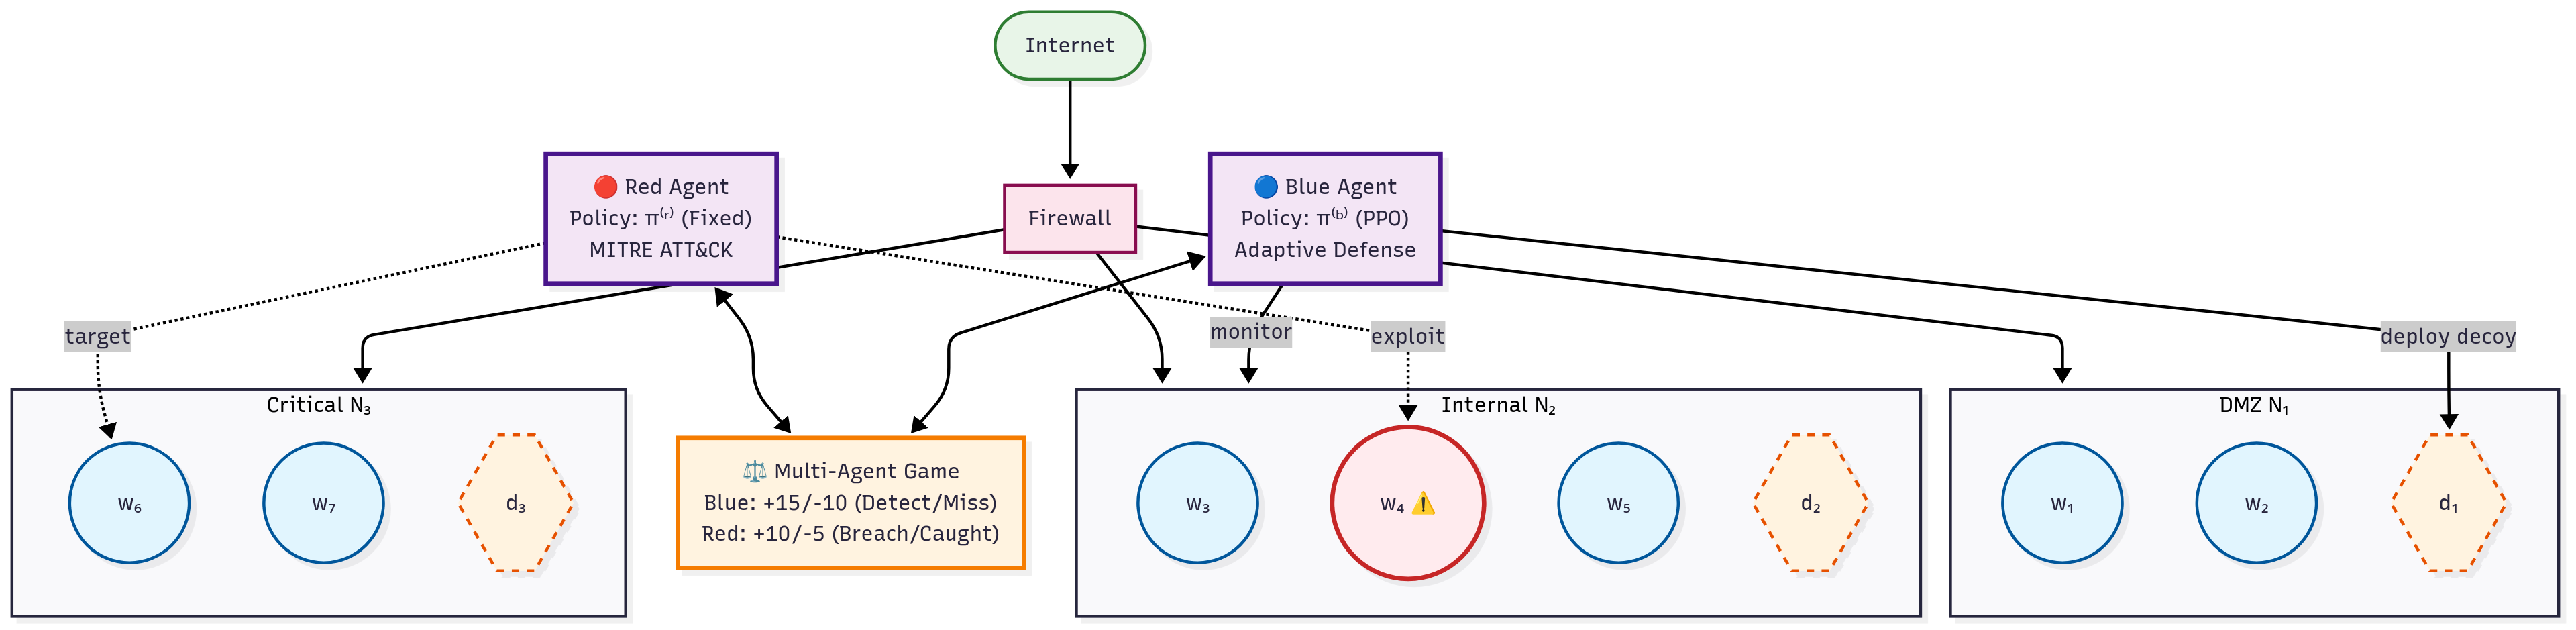
\includegraphics[width=0.8\textwidth]{figures/network_environment_mermaid.png}
%\caption{Alternative visualization: Multi-agent cyber defense environment using Mermaid-style representation showing the same network topology with enhanced visual clarity.}
%\label{fig:network_environment_mermaid}
%\end{figure}


\begin{figure}[H]
\centering
\begin{tikzpicture}[
    host/.style={circle, draw=blue!60, fill=blue!15, minimum size=7mm, font=\scriptsize, thick},
    decoy/.style={circle, draw=orange!70, fill=orange!15, minimum size=7mm, font=\scriptsize, thick, dashed},
    compromised/.style={circle, draw=red!70, fill=red!20, minimum size=7mm, font=\scriptsize, thick},
    subnet/.style={rectangle, draw=gray!50, fill=gray!8, minimum width=25mm, minimum height=20mm, thick, rounded corners=4pt, dashed},
    agentRed/.style={rectangle, draw=red!70, fill=red!15, minimum width=22mm, minimum height=12mm, font=\scriptsize, ultra thick, rounded corners=3pt},
    agentBlue/.style={rectangle, draw=blue!70, fill=blue!15, minimum width=22mm, minimum height=12mm, font=\scriptsize, ultra thick, rounded corners=3pt},
    firewall/.style={rectangle, draw=red!80, fill=red!20, minimum width=8mm, minimum height=15mm, font=\tiny, thick},
    internet/.style={ellipse, draw=green!60, fill=green!10, minimum width=20mm, minimum height=12mm, thick, align=center, font=\scriptsize}
]

% Internet - top left
\node[internet] (internet) at (-6, 6.5) {Internet};

% Firewall
\node[firewall] (firewall) at (-4, 6.5) {FW};

% Subnets - better spacing to avoid overlaps
\node[subnet] (subnet1) at (-5, 4) {};
\node[subnet] (subnet2) at (-1, 4) {};
\node[subnet] (subnet3) at (3, 4) {};

% Subnet labels - positioned clearly below subnets
\node[font=\small] at (-5, 2.8) {DMZ $N_1$};
\node[font=\small] at (-1, 2.8) {Internal $N_2$};
\node[font=\small] at (3, 2.8) {Critical $N_3$};

% Hosts - properly positioned within subnets
\node[host] (h1) at (-5.6, 4.3) {$w_1$};
\node[decoy] (d1) at (-4.4, 4.3) {$d_1$};

\node[host] (h2) at (-1.6, 4.3) {$w_2$};
\node[compromised] (h3) at (-0.4, 4.3) {$w_3$};

\node[host] (h4) at (2.4, 4.3) {$w_4$};
\node[host] (h5) at (3.6, 4.3) {$w_5$};

% Network backbone - adjusted positioning
\draw[thick, gray!60] (internet) -- (firewall);
\draw[thick, gray!60] (firewall) -- (-5, 3.2) -- (-1, 3.2) -- (3, 3.2);

% Internal Network label - positioned to avoid subnet overlap
\node[font=\small] at (-1, 2.4) {Internal Network};

% Agents - positioned lower to avoid overlap
\node[agentRed, align=center] (red) at (-5, 0.8) {\textbf{Red Agent}\\\textbf{Fixed} $\pi^{(r)}$};
\node[agentBlue, align=center] (blue) at (3, 0.8) {\textbf{Blue Agent}\\\textbf{PPO} $\pi^{(b)}$};

% Interactions with better label positioning
\draw[->, thick, blue!70] (blue) to[out=120, in=270] (d1);
\node[font=\tiny, blue!70] at (1.5, 2) {deploy};

\draw[->, thick, red!70, dashed] (red) to[out=60, in=270] (h3);
\node[font=\tiny, red!70] at (-2.5, 2) {attack};

% State/Info - positioned to avoid overlap
%\node[font=\tiny] at (-5, 0.1) {MITRE ATT\&CK};
%\node[font=\tiny, align=center] at (3, 0.1) {$d_b = %2|\mathcal{W}| + |\mathcal{N}||\mathcal{D}| + 2$};

% Essential state info
\node[font=\tiny] at (-5, 0.01) {MITRE ATT\&CK};
\node[font=\tiny] at (3, 0.01) {$d_b = 2|\mathcal{H}| + 2$};

% Rewards - positioned lower
\node[rectangle, draw=orange!70, fill=orange!10, minimum width=50mm, minimum height=15mm, rounded corners=3pt] (reward) at (-1, -1.2) {};
\node[font=\small, align=center] at (reward.center) {\textbf{Adversarial Rewards}\\Blue: +15/-10 \quad Red: +10/-5};

% Reward arrows
\draw[<->, orange!70, thick] (red.south) to[out=270, in=180] (reward.west);
\draw[<->, orange!70, thick] (blue.south) to[out=270, in=0] (reward.east);

\node[font=\scriptsize] at (6, 3.5) {\textbf{Legend}};
\node[host] at (5.2, 3.1) {}; \node[right, font=\scriptsize] at (5.5, 3.1) {Clean Host};
\node[decoy] at (5.2, 2.8) {}; \node[right, font=\scriptsize] at (5.5, 2.8) {Decoy Host};
\node[compromised] at (5.2, 2.5) {}; \node[right, font=\scriptsize] at (5.5, 2.5) {Compromised};
%\node[firewall] at (5.2, 2.2) {}; \node[right, font=\scriptsize] at (5.5, 2.2) {Firewall};

% Environment scale
\node[font=\tiny, align=center] at (6, 1.5) {Scale:\\15-200 hosts\\3-8 subnets};

\end{tikzpicture}
\caption{Multi-agent cyber defense environment showing DMZ and internal subnets containing real assets and decoys. Red agent executes attacks with MITRE ATT\&CK (dashed red arrows) while Blue agent learns optimal decoy deployment with PPO (solid blue arrows). Rewards provide feedback for learning.}
\label{fig:network_environment}
\end{figure}


\subsubsection{Mathematical Foundation}
The network environment is represented as a directed graph $G = (V, E)$:

\begin{align}
G &= (V, E) \text{ where } G = \text{nx.DiGraph}() \\
V &= \mathcal{W} \cup \mathcal{N} \cup \mathcal{R}_{net} \\
E &\subseteq V \times V
\end{align}

where $\mathcal{W}$ represents hosts (computers/devices), $\mathcal{N}$ represents subnets, $\mathcal{R}_{net}$ represents routers, and $E$ represents directed network connections.

Each host $w_i \in \mathcal{W}$ is characterized by a comprehensive state vector:
\begin{equation}
w_i = \langle \text{IP}_i, \text{OS}_i, \text{Services}_i, \text{Vulns}_i, \text{is\_compromised}_i, \text{decoy}_i \rangle
\end{equation}

where $\text{IP}_i$ is the IP address, $\text{OS}_i$ is the operating system, $\text{Services}_i$ are running services, $\text{Vulns}_i$ are vulnerabilities, $\text{is\_compromised}_i \in \{0,1\}$ indicates compromise status, and $\text{decoy}_i \in \{0,1\}$ indicates whether the host is a honeypot.

\subsubsection{Implementation Details}
\paragraph{The environment is implemented with these details.}The architecture uses \texttt{nx.DiGraph} directed graph structure with scale support for larger networks, the validated empirical range for this research covers 15-200 hosts. MITRE integration implements 7 kill-chain phase techniques following the ATT\&CK methodology through YAML-driven modularity across all components.

Having established the network environment representation, we now detail the specific agent implementations operating within this framework, beginning with the adversarial red agent.

\subsection{Red Agent (Fixed Adversary)}

The red agent serves as a fixed, pre-trained cyber adversary implementing MITRE ATT\&CK framework patterns. It provides consistent adversarial pressure essential for reproducible defensive training and evaluation.

\subsubsection{Attack Behavior}
The red agent executes a structured kill chain that progresses through discovery via network scanning and reconnaissance, followed by exploitation to compromise vulnerable hosts. Once established, the agent performs lateral movement to spread throughout the network from its initial foothold, ultimately attempting to achieve impact on target systems. This deterministic progression ensures reproducible attack scenarios that enable fair comparison of defensive strategies across experiments.

\subsubsection{Role in Defensive Training}
The fixed adversary design provides essential benefits for rigorous experimental evaluation. Standardized attack patterns enable controlled comparison of blue agent performance without the confounding variables introduced by adaptive opponents. The MITRE ATT\&CK-based progression reflects real-world attack sophistication while maintaining experimental reproducibility. Most importantly, the fixed opponent eliminates co-evolution complexity, allowing us to isolate defensive learning dynamics and focus specifically on blue agent adaptation without concurrent adversarial learning.

\subsubsection{State Space and Actions}

The red agent maintains situational awareness through structured internal state tracking rather than a single observation vector. At each timestep $t$, the agent's knowledge consists of its current position $\text{current\_host}_t \in \mathcal{W}$, accumulated network intelligence through $\text{history}_t$, and detailed reconnaissance data about discovered hosts in $\text{tracked\_hosts}_t \subseteq \mathcal{W}$. This internal state representation can be formalized as:

\begin{equation}
\mathcal{S}^{(r)}_t = \{\text{current\_host}_t, \text{history}_t, \text{tracked\_hosts}_t, \text{services\_map}_t, \text{unimpacted\_hosts}_t\}
\end{equation}

The agent's operational capabilities expand dynamically as network knowledge grows. Each discovered host becomes a potential target for the seven-phase MITRE ATT\&CK kill chain $\mathcal{K} = \{\text{pingsweep}, \text{portscan}, \text{discovery}, \text{lateral-movement}, \text{privilege-escalation}, \text{impact}, \text{nothing}\}$. The action space at timestep $t$ reflects this reconnaissance-driven expansion:

\begin{equation}
\mathcal{A}^{(r)}_t = \mathcal{K} \times \text{tracked\_hosts}_t \quad \text{with size} \quad |\mathcal{A}^{(r)}_t| = 7 \times |\text{tracked\_hosts}_t|
\end{equation}

This formulation captures the adaptive nature of cyber attacks, where an adversary's capabilities grow through successful reconnaissance and network mapping activities.

The adversarial learning framework is illustrated in Figure~\ref{fig:adversarial_framework}.

\begin{figure}[H]
\centering
\textbf{Adversarial Learning Framework}
\medskip
\begin{adjustbox}{max width=0.95\linewidth,center}
\begin{tikzpicture}[font=\footnotesize,node distance=2.5cm,box/.style={draw=black,rounded corners,minimum width=3.2cm,minimum height=1.5cm,align=center,fill=white,thick}]
    % Nodes with slightly better spacing and sizing
    \node[box,fill=red!25] at (0,0) (redA) {\textbf{Red}\\$\pi^{(r)}$ (fixed)};
    \node[box,fill=blue!15] at (6,0) (env) {\textbf{Environment}\\State $S_t$\\Attack Surface};
    \node[box,fill=green!20] at (12,0) (blueA) {\textbf{Blue}\\$\pi_\theta$ (PPO)};
    
    \draw[->,very thick,red!80] (redA) -- node[above,font=\scriptsize,red!80]{Actions} (env);
    \draw[->,very thick,blue!80] (env) -- node[above,font=\scriptsize,blue!80]{Obs.} (blueA);
    \draw[->,very thick,black] (blueA) to[out=210,in=330] node[below,font=\scriptsize,black]{Defense} (env);
    \draw[->,very thick,red!80] (env) to[out=30,in=150] node[above,font=\scriptsize,red!80]{Reward} (blueA);
    \draw[->,very thick,black!70] (env) to[out=210,in=-30] node[below,font=\scriptsize,black!70]{State $\Delta$} (redA);
\end{tikzpicture}
\end{adjustbox}
\caption{Adversarial Learning Loop. The fixed red agent policy produces consistent attack actions, the environment state gets updated, and the blue agent receives observations and rewards, and learns adaptive defensive strategies through PPO. The environment facilitates this adversarial interaction and learning signal generation}
\label{fig:adversarial_framework}
\end{figure}




\subsection{Blue Agent (Learnable Defender)}

The blue agent implements adaptive defensive strategies emphasizing cyber deception and strategic network isolation through PPO-based reinforcement learning.

\subsubsection{State Space and Observations}

The blue agent's state space $S^{(b)}_t \in \mathbb{R}^{d_b}$ has a simplified observation structure:

\begin{equation}
S^{(b)}_t = \begin{bmatrix}
\text{current\_alerts}_t \\
\text{alert\_history}_t \\
\text{metadata}_t
\end{bmatrix}
\end{equation}

where $\text{current\_alerts}_t \in \{0,1\}^{|\mathcal{W}|}$ represents immediate threat indicators per host, $\text{alert\_history}_t \in \{0,1\}^{|\mathcal{W}|}$ captures cumulative attack memory enabling pattern learning, and $\text{metadata}_t \in \mathbb{R}^2$ contains environmental constants: a fixed value of $-1$ and the total number of active decoys.

\textbf{State Space Dimensionality Analysis}

The total dimensionality is $d_b = 2|\mathcal{W}| + 2$, comprising alert components with $2|\mathcal{W}|$ dimensions (current + historical per host) and metadata components with $2$ dimensions (environmental constants: fixed value $-1$ and total decoy count).

This structure enables both immediate threat response and strategic pattern learning. Figure~\ref{fig:observation_vector} provides a detailed breakdown of the observation vector structure and dimensionality.

% Enhanced observation_vector figure matching comprehensive layout design
\begin{figure}[htbp]
\centering
\begin{tikzpicture}[node distance=0.3cm and 0.8cm, every node/.style={font=\small}]

    % Refined styles for optimal presentation
    \tikzset{
        vectorbox/.style={draw=black, rounded corners=3pt, fill=white, inner sep=8pt, minimum width=3.2cm, minimum height=2.0cm, align=center, thick, text width=3.0cm},
        totalsection/.style={draw=black, rounded corners=3pt, fill=gray!10, inner sep=10pt, minimum width=13cm, align=center, thick},
        arrow/.style={->, thick, black, >=stealth, line width=1pt},
        dimension/.style={font=\footnotesize\ttfamily, color=blue!70!black}
    }

    % Main vector components in horizontal layout
    \node[vectorbox, fill=red!15] (current) {
        \textbf{Current Alerts}\\
        \textcolor{blue!70!black}{$|\mathcal{W}|$ dimensions}\\
        \footnotesize immediate threat detection\\
        \footnotesize per host
    };
    
    \node[vectorbox, fill=blue!15, right=of current] (historical) {
        \textbf{Historical Alerts}\\
        \textcolor{blue!70!black}{$|\mathcal{W}|$ dimensions}\\
        \footnotesize temporal pattern learning\\
        \footnotesize sticky memory
    };
    
    \node[vectorbox, fill=green!15, right=of historical] (padding) {
        \textbf{Padding}\\
        \textcolor{blue!70!black}{1 dimension}\\
        \footnotesize Vector alignment\\
        \footnotesize and structure
    };
    
    \node[vectorbox, fill=yellow!15, right=of padding] (decoy) {
        \textbf{Decoy Count}\\
        \textcolor{blue!70!black}{1 dimension}\\
        \footnotesize Strategic context\\
        \footnotesize and deception
    };

    % Total dimension summary
    \node[totalsection, below=1.5cm of historical] (total) {
        \textbf{Total Dimension: }$d_b = 2|\mathcal{W}| + 2$\\
        \footnotesize Host-aligned alert segments + metadata for\\
        \footnotesize comprehensive strategic decision-making\\
        \footnotesize Improved layout prevents text overlap and enhances readability\\
        \footnotesize with better spacing and color contrast.
    };

    % Connection arrows showing information flow
    \draw[arrow] (current.south) -- ++(0,-0.4) -| (total.north west);
    \draw[arrow] (historical.south) -- ++(0,-0.7) -- (total.north);
    \draw[arrow] (padding.south) -- ++(0,-0.4) -| (total.north east);
    \draw[arrow] (decoy.south) -- ++(0,-0.2) -| (total.north east);

\end{tikzpicture}
\caption{Blue Observation Vector Structure: Comprehensive state representation with current alerts, historical patterns, padding for alignment, and decoy count for strategic context. Improved layout prevents text overlap and enhances readability with better spacing and color contrast.}
\label{fig:observation_vector}
\end{figure}

\subsubsection{Action Space and Defense Operations}

The blue agent's action space consists of defensive operations implemented as a discrete action space:

\begin{equation}
\mathcal{A}^{(b)} = \mathcal{A}_{\text{deploy}} \cup \mathcal{A}_{\text{remove}} \cup \{\text{nothing}\}
\end{equation}

where $\mathcal{A}_{\text{deploy}} = \{(\text{deploy\_decoy}, n_j) : n_j \in \mathcal{N}\}$ deploys a decoy on subnet $n_j$, $\mathcal{A}_{\text{remove}} = \{(\text{remove\_decoy}, n_j) : n_j \in \mathcal{N}\}$ removes a decoy from subnet $n_j$, and $\text{nothing}$ represents no action (observation only).

Total action space size: $|\mathcal{A}^{(b)}| = 2|\mathcal{N}| + 1$.

\subsection{Reward System: Mathematical Relationships and Timing}

This section establishes unified notation and explicit mathematical relationships between red and blue rewards.

\textbf{Fundamental Reward Structure}

Our system implements a \textbf{competitive reward structure} where red and blue agents have opposing objectives, formalized as:

\begin{equation}
R^{(b)}_t + R^{(r)}_t = C - \text{system\_costs}_t
\end{equation}

where $C$ is a normalization constant and system costs represent computational overhead. This creates a near-zero-sum game where blue agent success directly corresponds to red agent failure.

\textbf{Red Agent Reward Components}

The red agent reward function is determined by the specific action executed, with rewards configured per action type as shown in the actual implementation.

\textbf{Blue Agent Reward Components}

The blue agent reward function emphasizes deception effectiveness through a 10× multiplier when red agents attack decoys, while imposing negative rewards when real hosts are compromised. Additional costs are applied for deployment and removal actions as configured.

\textbf{Unified Mathematical Relationship}

The competitive relationship is implemented through direct coupling of red and blue rewards based on action outcomes and target types, as described in the implemented reward functions above.

\textbf{Shared Outcome Variables}: Both reward functions depend on common environmental variables including $\mathbf{1}[\text{technique}_i \text{ successful}]$ used in both $R^{(r)}_t$ and $R^{(b)}_t$ calculations, $\Delta\text{assets\_compromised}_t$ where direct red gain becomes direct blue loss, and $\mathbf{1}[\text{detected}_t]$ where red penalty corresponds to blue monitoring success.

\textbf{Reward Timing and Detection Mechanisms}

\textit{Detection Timing}: Rewards are computed immediately following each agent action based on the resulting environment state. Detection occurs when red agent actions trigger alert thresholds in the monitoring system, blue agent observes attack signatures in current observation vector, or decoy interactions generate immediate deception reward signals.

\textit{Multi-step Effects}: While immediate rewards capture direct action consequences, our reward structure also accounts for delayed effects through the temporal discount factor $\gamma = 0.99$, allowing agents to learn multi-step strategies where early actions enable later tactical advantages.

\textit{Detection Delay Modeling}: In our current implementation, detection is modeled as immediate for computational tractability. However, the framework accommodates delayed detection through state history mechanisms where attack indicators persist across multiple time steps before triggering alerts.

\textbf{Unified Mathematical Formulation with Specific Parameter Values}

Building on the mathematical relationships above, we provide the specific instantiation used in our experiments:

Let $\mathcal{N}_t = \{w_1, w_2, \ldots, h_n\}$ be the network state at time $t$, where each host $w_i$ has status $\sigma_i \in \{\text{clean}, \text{compromised}, \text{decoy}\}$. 

Define detection events:
\begin{align}
D_t^{\text{decoy}} &= \mathbb{I}[\text{red attacks decoy at time } t] \\
D_t^{\text{real}} &= \mathbb{I}[\text{red attacks real host at time } t] \\
D_t^{\text{success}} &= \mathbb{I}[\text{red successfully compromises new host at time } t]
\end{align}

\textbf{Blue Agent Reward Function} $R_t^{(b)}$ (Implemented):
\begin{align}
R_t^{(b)} = \begin{cases}
\text{red\_reward} \times 10 & \text{if red attacks decoy successfully} \\
-\text{red\_reward} & \text{if red attacks real host successfully} \\
\text{blue\_action\_reward} & \text{if blue action succeeds} \\
0 & \text{otherwise}
\end{cases} + \text{recurring\_rewards}
\end{align}

where the specific reward values from configuration are: deploy\_decoy immediate reward = $-20.0$, remove\_decoy immediate reward = $-1.0$, nothing immediate reward = $0.0$, and red\_reward values are determined by the red agent's action configuration. The reward calculation emphasizes deception success (10× multiplier) over deployment costs.

\textbf{Red Agent Reward Function} $R_t^{(r)}$ (Fixed Adversary):
Since the red agent operates as a fixed adversary with deterministic strategy, its reward is determined by the action executed:
\begin{equation}
R_t^{(r)} = \text{immediate\_reward}[\text{action}] + \text{recurring\_reward}[\text{action}]
\end{equation}

where the specific reward values from configuration are: pingsweep = $1$, portscan = $2$, discovery = $5$, lateral-movement = $10$, privilege-escalation = $20$, impact = $50$, nothing = $0$. All recurring rewards are $0$.

\textbf{Adversarial Reward Properties}:
The reward functions exhibit adversarial properties in key interaction scenarios based on actual implementation:
\begin{align}
\text{When red attacks decoy:} \quad R_t^{(b)} &= +\text{red\_reward} \times 10 \\
R_t^{(r)} &= +\text{red\_reward} \text{ (action-specific)} \\
\text{When red attacks real host:} \quad R_t^{(b)} &= -\text{red\_reward} \\
R_t^{(r)} &= +\text{red\_reward} \text{ (action-specific)}
\end{align}

\textbf{RL Optimization Objective}:
Since only the blue agent learns (red agent is fixed), the learning objective is:
\begin{align}
J^{(b)} &= \mathbb{E}\left[\sum_{t=1}^{T} \sum_{h=1}^{H} \gamma^{h-1} R_h^{(b)}\right]
\end{align}
where the blue agent optimizes this objective using PPO while the red agent follows a fixed deterministic strategy.

where $\gamma = 0.99$ is the discount factor, $T$ is the number of trials, and $H$ is the episode horizon.

\subsubsection{Environment-Agent Interaction Dynamics}

\begin{figure}[H]
\centering
\textbf{Environment--Agent Interaction}
\medskip
\begin{adjustbox}{max width=0.95\linewidth,center}
\begin{tikzpicture}[font=\footnotesize,node distance=1.9cm,sys/.style={draw=black,rounded corners,minimum width=3.2cm,minimum height=1.7cm,align=center,fill=white}]
    % Nodes tightened
    \node[sys,fill=red!25] at (0,0) (red) {\textbf{Red}\\$\pi^{(r)}$ fixed};
    \node[sys,fill=blue!12] at (5.1,0) (envInt) {\textbf{Env. $\MC{E}$}\\Hosts $\mathcal{N}_t$\\Decoys $\mathcal{D}_t$};
    \node[sys,fill=green!18] at (10.2,0) (blue) {\textbf{Blue}\\PPO $\pi_\theta$};
    % Arrows
    \draw[->,very thick,red] (red) -- node[above,font=\scriptsize]{Attacks} (envInt);
    \draw[->,very thick,blue] (envInt) -- node[above,font=\scriptsize]{Obs.} (blue);
    \draw[->,very thick,black] (blue) to[out=150,in=30] node[above,font=\scriptsize]{Def. Actions} (envInt);
    % Signals ellipse condensed
    \node[draw,ellipse,fill=gray!10,inner sep=2pt,below=0.9cm of envInt] (signals) {Det./Comp. Signals};
    \draw[-latex,thick] (envInt.south) -- (signals.north);
    \draw[-latex,thick] (signals.west) -- +( -0.9,0) node[left,font=\tiny]{Reward Terms};
    \draw[-latex,thick] (signals.east) -- +( 0.9,0) node[right,font=\tiny]{Shaping};
\end{tikzpicture}
\end{adjustbox}
\caption{Tightened interaction loop: red produces attacks, environment updates host/decoy state, blue observes and deploys/removes decoys, signals feed reward.}
\label{fig:environment_interaction}
\end{figure}

\begin{enumerate}
\item \textbf{Action-Reward Causality}: Rewards are triggered by specific detection events within the same timestep as actions
\item \textbf{Detection Mechanism}: $D_t^{\text{decoy}}$ and $D_t^{\text{success}}$ are determined by red agent actions interacting with current network state $\mathcal{N}_t$
\item \textbf{Temporal Consistency}: All reward components $R_t^{(b)}$ are observed immediately at time $t$, eliminating credit assignment ambiguity
\item \textbf{Causality Chain}: Blue action at $t-1$ modifies $\mathcal{N}_t$ → Red action at $t$ triggers detection → Rewards observed at $t$
\end{enumerate}

\textbf{Learning Signal Properties}: This unified formulation provides PPO with consistent variables where all reward terms use the same mathematical framework and timing, clear adversarial structure through explicit zero-sum relationships in key interaction scenarios, temporal precision via exact specification of when rewards are observed relative to actions, and strategic incentives where $\alpha_2 \gg \alpha_1$ encourages strategic deception over reactive deployment.


\subsection{Environment Selection and Extensibility Rationale}

\textbf{Why Cyberwheel?} The Cyberwheel framework was developed by Oak Ridge National Laboratory (ORNL) as a modular, extensible platform for cybersecurity research and was selected after comparative review of alternative cyber-range simulation environments (e.g., CybORG, CAGE, OpenAI Gym network extensions) based on three key advantages: (1) \textbf{native deception support} for decoy deployment state transitions crucial to our research, (2) \textbf{modular YAML-driven configuration} enabling systematic experimentation and baseline comparison, and (3) \textbf{scalable architecture} supporting networks from 15 hosts to enterprise scale with deterministic adversary modes for controlled learning analysis.

\textbf{ORNL Repository and Development Context}: The original Cyberwheel framework and documentation are maintained by Oak Ridge National Laboratory, with development motivated by the need for reproducible, scalable cybersecurity RL research platforms. This aligns directly with our requirements for systematic baseline comparison and experimental rigor.

\textbf{Design Considerations}: Our experimental design focuses on establishing fundamental defensive learning behaviors using a fixed adversary model. This approach preserves interpretability of baseline defensive learning signals and enables systematic analysis of policy behavior without additional complexity from dynamic attacker adaptation, leveraging Cyberwheel's modular design for controlled experimental conditions.

\subsubsection{Cyberwheel Configuration System Architecture}

\begin{figure}[H]
\centering
\begin{tikzpicture}[scale=1.2,font=\tiny,node distance=1cm,transform shape]
    % Main Configuration Hierarchy
    \node[draw=cwBorder, thick, rounded corners, fill=cwFlow!15, text width=2.2cm, align=center] at (0,0) (root) {\textbf{Cyberwheel Config}\\YAML Hierarchy};
    
    % Environment Configuration
    \node[draw=cwDecoy!60, thick, rounded corners, fill=cwDecoy!15, text width=2cm, align=center] at (-2,-2) (env) {\textbf{Environment}\\Network topology\\Host configs\\Attack patterns};
    
    % Agent Configuration  
    \node[draw=cwAlert!60, thick, rounded corners, fill=cwAlert!15, text width=2cm, align=center] at (2,-2) (agent) {\textbf{Agent Config}\\PPO parameters\\Learning rates\\Net architecture};
    
    % Mathematical Mapping
    \node[draw=cwReal!60, thick, rounded corners, fill=cwReal!15, text width=2cm, align=center] at (0,-4) (math) {\textbf{Mathematical\\Mapping}\\$\gamma$, $\lambda$, $\epsilon$\\Formal verify};
    
    % Experimental Controls
    \node[draw=cwBorder!80, thick, rounded corners, fill=cwBorder!20, text width=2cm, align=center] at (-3,-4) (exp) {\textbf{Experimental\\Controls}\\Seeds: \{1,42,123...\}\\Fixed red policy\\Unified logging};
    
    % Implementation Verification
    \node[draw=cwBorder!80, thick, rounded corners, fill=cwBorder!20, text width=2cm, align=center] at (3,-4) (impl) {\textbf{Implementation\\Verification}\\Code-config map\\Parameter validation\\Baseline consistent};
    
    % Arrows
    \draw[-stealth, thick, cwFlow] (root) -- (env);
    \draw[-stealth, thick, cwAlert] (root) -- (agent);
    \draw[-stealth, thick, cwReal] (root) -- (math);
    \draw[-stealth, thick, cwDecoy] (env) -- (exp);
    \draw[-stealth, thick, cwAlert] (agent) -- (impl);
    \draw[-stealth, thick, cwReal] (math) -- (exp);
    \draw[-stealth, thick, cwReal] (math) -- (impl);
\end{tikzpicture}
\label{fig:config_architecture}

\caption{Cyberwheel Configuration System Architecture: YAML-driven modular design enables systematic experimental control through hierarchical parameter organization. Mathematical mapping ensures theoretical formulations align with implementation parameters, supporting reproducible comparative analysis.}
\end{figure}


\subsubsection{Unified Mathematical Notation}

We build on the problem formulation above to establish a comprehensive notation system used throughout this work:

\begin{table}[H]
\centering
\caption{Unified Mathematical Notation Framework}
\label{tab:unified_notation}
\small
\begin{tabular}{|l|l|p{6cm}|}
\hline
\textbf{Symbol} & \textbf{Domain} & \textbf{Definition} \\
\hline
\multicolumn{3}{|c|}{\textbf{Network Environment}} \\
\hline
$G = (V, E)$ & Topology & Directed graph representing network topology \\
$V$ & Vertices & Set of all graph vertices: $V = \mathcal{W} \cup \mathcal{N} \cup \mathcal{R}_{net}$ \\
$E$ & Edges & Set of directed network connections \\
$\mathcal{W} = \{w_1, \ldots, w_n\}$ & Hosts & Set of network hosts/devices \\
$\mathcal{N} = \{N_1, \ldots, N_k\}$ & Subnets & Set of network subnets \\
$\mathcal{R}_{net}$ & Routers & Set of network routing devices \\
$\mathcal{D}$ & Decoys & Set of available decoy types \\
$\mathcal{T}$ & Techniques & Set of MITRE ATT\&CK techniques (295 total) \\
\hline
\multicolumn{3}{|c|}{\textbf{Agent States \& Actions}} \\
\hline
$\mathcal{S}^{(r)}$ & Red Agent & Red agent internal state tracking (no explicit vector) \\
$\mathcal{S}^{(b)} \subset \mathbb{R}^{d_b}$ & Blue Agent & Blue agent state space \\
$d_b = 2|\mathcal{W}| + 2$ & Dimensions & Blue agent state space dimensionality \\
$\mathcal{A}^{(r)}$ & Red Agent & Red agent action space (7 MITRE ATT\&CK actions per known host) \\
$\mathcal{A}^{(b)}$ & Blue Agent & Blue agent action space (deploy/remove decoys per subnet + nothing) \\
$S_t^{(r)}, S_t^{(b)}$ & States & Agent states at timestep $t$ \\
$A_t^{(r)}, A_t^{(b)}$ & Actions & Agent actions at timestep $t$ \\
\hline
\multicolumn{3}{|c|}{\textbf{Policies \& Learning}} \\
\hline
$\pi^{(r)}_{\text{fixed}}$ & Red Agent & Fixed deterministic red policy \\
$\pi^{(b)}$ & Blue Agent & Learnable blue policy (PPO) \\
$J^{(b)}(\pi^{(b)})$ & Objective & Blue agent learning objective \\
$H$ & Episodes & Maximum episode length (time steps) \\
$T$ & Training & Total number of training episodes \\
$t$ & Time & Current timestep within episode \\
$\gamma$ & Learning & Discount factor (0.99) \\
\hline
\multicolumn{3}{|c|}{\textbf{Rewards}} \\
\hline
$R_t^{(r)}, R_t^{(b)}$ & Rewards & Immediate rewards at timestep $t$ \\
$\mathcal{R}^{(r)}, \mathcal{R}^{(b)}$ & Functions & Reward functions \\
\multicolumn{3}{|c|}{\textbf{Actual Reward Values (from configuration)}} \\
\hline
\textbf{Red Action Rewards} & Values & pingsweep=1, portscan=2, discovery=5, lateral-movement=10, privilege-escalation=20, impact=50, nothing=0 \\
\textbf{Blue Action Rewards} & Values & deploy\_decoy=-20.0, remove\_decoy=-1.0, nothing=0.0 \\
\textbf{Deception Multiplier} & Blue & Red reward × 10 when attacking decoys \\
\textbf{Compromise Penalty} & Blue & -Red reward when attacking real hosts \\
\hline
\end{tabular}
\end{table}

Having established the mathematical framework above, we now describe how this formulation maps to realistic network environments and the specific state space representations used by both agents.
\subsection{Configuration--Mathematical Parameter Mapping}

Table~\ref{tab:config_mapping} links symbolic notation used in formal definitions to concrete configuration sources. Only parameters present in the current codebase are listed; unimplemented or future-planned elements are omitted.

\begin{table}[H]
\centering
\caption{Mathematical Notation Framework: Mapping of symbols to configuration fields and implementation details}
\label{tab:config_mapping}
\begin{tabular}{lllp{5.5cm}}
\rowcolor{cwBorder!30} \textbf{Symbol} & \textbf{Name} & \textbf{Config Source} & \textbf{Role} \\
\midrule
$\gamma$ & Discount Factor & rl/ppo yaml & Temporal weighting of future rewards (set 0.99) \\
$\lambda$ & GAE Parameter & rl/ppo yaml & Bias--variance trade-off in advantage estimation (set 0.95) \\
$\epsilon$ & PPO Clip Range & rl/ppo yaml & Trust region style constraint (set 0.2) \\
$c_1$ & Entropy Coefficient & rl/ppo yaml & Encourages exploration (set 0.01) \\
$c_2$ & Value Loss Coefficient & rl/ppo yaml & Balances policy vs critic optimization (set 0.5) \\
$|\mathcal{W}|$ & Host Count & topology yaml & Defines alert vector segments / state dimensionality \\
$|\mathcal{N}|$ & Subnet Count & topology yaml & Determines action mapping size (deploy/remove granularity) \\
$H$ & Episode Horizon & env settings & Upper bound on per-episode decision steps \\
$T$ & Training Episodes & run script args & Outer loop sample budget controlling convergence window \\
$\alpha_{1..4}$ & Reward Weights & reward module & Shape deployment, deception, compromise, removal incentives \\
$\beta_{1},\beta_{2}$ & Red Reward Weights & reward module & Maintain adversarial structure (fixed opponent accounting) \\
\bottomrule
\end{tabular}
\end{table}

\end{document}